\begin{figure}[ht]
\centering
% Thesis-wide categorical color palette
% Usage: % Thesis-wide categorical color palette
% Usage: % Thesis-wide categorical color palette
% Usage: \input{figures/palette} in any figure file
%
% Muted primary colors -- print-friendly, visually distinct.
% Inspired by Cooper Union's red/blue primaries, softened for
% academic figures. Use palA-palC for data series in scatter
% plots, line charts, bar charts, etc.

\definecolor{palA}{HTML}{1F77B4}   % Tableau blue
\definecolor{palB}{HTML}{D62728}   % Tableau red
\definecolor{palC}{HTML}{2CA02C}   % Tableau green
 in any figure file
%
% Muted primary colors -- print-friendly, visually distinct.
% Inspired by Cooper Union's red/blue primaries, softened for
% academic figures. Use palA-palC for data series in scatter
% plots, line charts, bar charts, etc.

\definecolor{palA}{HTML}{1F77B4}   % Tableau blue
\definecolor{palB}{HTML}{D62728}   % Tableau red
\definecolor{palC}{HTML}{2CA02C}   % Tableau green
 in any figure file
%
% Muted primary colors -- print-friendly, visually distinct.
% Inspired by Cooper Union's red/blue primaries, softened for
% academic figures. Use palA-palC for data series in scatter
% plots, line charts, bar charts, etc.

\definecolor{palA}{HTML}{1F77B4}   % Tableau blue
\definecolor{palB}{HTML}{D62728}   % Tableau red
\definecolor{palC}{HTML}{2CA02C}   % Tableau green

\definecolor{encfade}{HTML}{B8D2E6}
\definecolor{reprfill}{HTML}{D6E8F4}
\definecolor{headfill}{HTML}{E8E8E8}
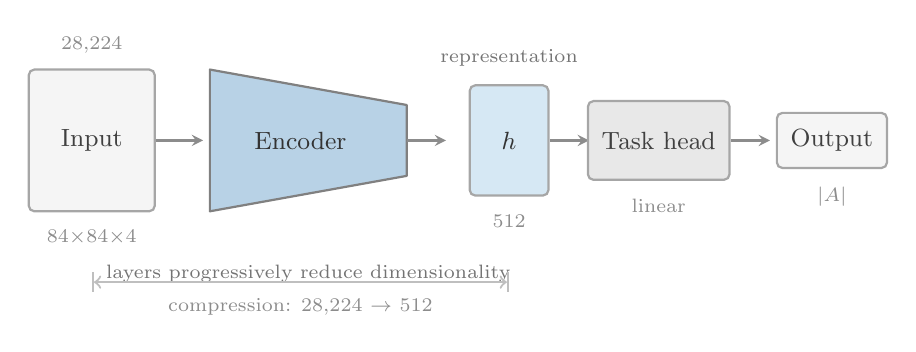
\begin{tikzpicture}[
    arr/.style={->, thick, >=stealth, black!45},
    lbl/.style={font=\small, text=black!80},
    dimlbl/.style={font=\scriptsize, text=black!45},
    sublbl/.style={font=\scriptsize, text=black!55},
    block/.style={draw=black!35, thick, rounded corners=2pt,
                  minimum height=0.8cm, font=\small,
                  text=black!75, inner sep=5pt},
]

% --- Input ---
\node[block, fill=black!4, minimum width=1.6cm,
      minimum height=1.8cm] (input) at (0, 0) {Input};
\node[dimlbl, below=3pt] at (input.south) {$84{\times}84{\times}4$};
\node[dimlbl, above=2pt] at (input.north) {28{,}224};

\draw[arr] (input.east) -- ++(0.6, 0);

% --- Encoder (trapezoid matching single-objective.tex) ---
\fill[encfade, draw=black!50, thick, line join=round]
    (1.5, -0.9) -- (1.5, 0.9) -- (4.0, 0.45) -- (4.0, -0.45)
    -- cycle;
\node[lbl] at (2.65, 0) {Encoder};
\node[sublbl, below=16pt] at (2.75, -0.9) {layers progressively
    reduce dimensionality};

\draw[arr] (4.0, 0) -- ++(0.5, 0);

% --- Representation (bottleneck) ---
\node[block, fill=reprfill, minimum width=1.0cm,
      minimum height=1.4cm, text=black!80,
      font=\small\bfseries] (repr) at (5.3, 0) {$h$};
\node[dimlbl, below=3pt] at (repr.south) {512};
\node[sublbl, above=3pt] at (repr.north) {representation};

\draw[arr] (repr.east) -- ++(0.5, 0);

% --- Task head ---
\node[block, fill=headfill, minimum width=1.2cm,
      minimum height=1.0cm] (head) at (7.2, 0) {Task head};
\node[dimlbl, below=3pt] at (head.south) {linear};

\draw[arr] (head.east) -- ++(0.5, 0);

% --- Output ---
\node[block, fill=black!4, minimum width=1.0cm,
      minimum height=0.7cm] (output) at (9.4, 0) {Output};
\node[dimlbl, below=3pt] at (output.south) {$|A|$};

% --- Dimensionality annotation (spanning arrow) ---
\draw[black!25, thick, |<->|]
    (0, -1.8) -- (5.3, -1.8)
    node[midway, below=2pt, dimlbl] {compression:
    28{,}224 $\to$ 512};

\end{tikzpicture}
\caption{Encoder, representation, and task head. The encoder
  compresses a high-dimensional input into a low-dimensional
  representation~$h$. The task head reads from this representation
  to produce the output. The same pattern appears in DQN
  (\cref{sec:dqn}), where the encoder is a convolutional network
  and the task head maps representations to Q-values.}
\label{fig:encoder-latent-space}
\end{figure}
